\section{VQ-VAE}
\label{sec:vqvae}

Vector Quantized Variational Autoencoder (VQ-VAE) \cite{vqvae} is a generative models based on VAE \ref{sec:vae} model with the addition of vector quantization (VQ) (section \ref{subsec:vqvae_vq}) technique. 

\subsection{Vector Quantization}
\label{subsec:vqvae_vq}

Vector quantization (VQ) is a technique used to discretize continuous data. In the context of VQ-VAE, the continuous latent space $z$ is mapped into discrete codes vectors. In a continuous latent space, the amount of possibilities for a value in the hidden space is infinite, which makes it difficult for the model to learn the hidden space efficiently. With a discrete hidden space, learning becomes more efficient because there is a fixed number of possible values (although in reality it is very large, for example the amount of objects that can be described using language is finite but very large). Furthermore, in reality, images are divided into classes of objects such as cats, people, dogs, etc., and each class has a finite number of possibilities, which is better suited to a discrete latent vectors.

\begin{figure}[h]
    \centering
    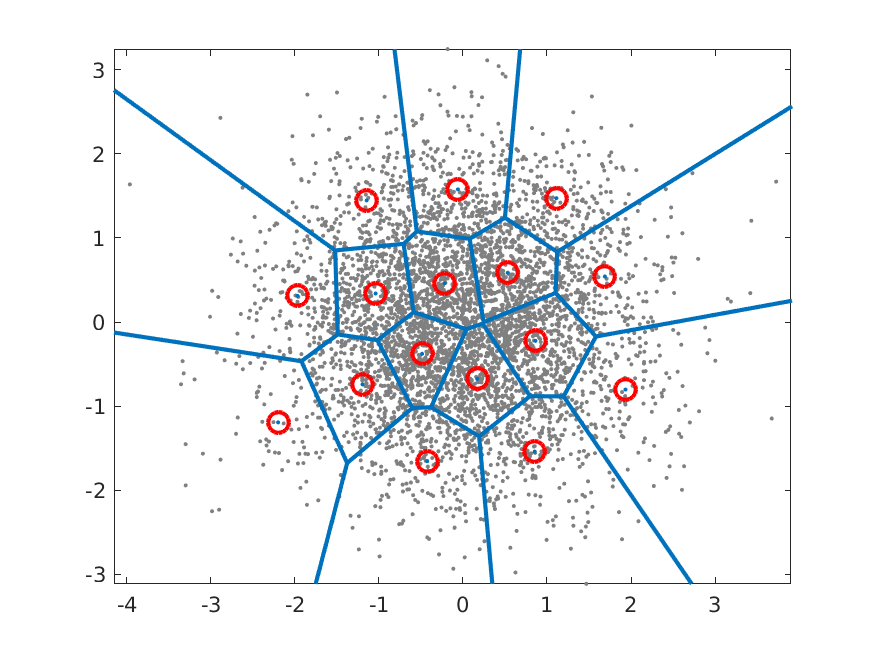
\includegraphics[scale=0.5]{images/vq_visualization.png}
    \caption{Illustration of vector quantization discrete clustering of the 2D latent space \cite{vq_visualization_website}. The grey dots are embeddings of the continous latent space, and the red dots are the code vectors from the codebook. In this case, the codebook size is 16.}
    \label{figure:vq_visualization}
\end{figure}

This technique involves the use of a codebook, which is a discrete collection of vectors of the same size as the hidden dimension. In the VQ-VAE model, after the input passes through the encoder (which results in embeddings - which are the hidden representation of the input), the embeddings are replaced by the closest vector from the codebook (by minimizing distance between vectors). This operation allows the model to learn clusters of similar embeddings, which can be used to generate new samples. The codebook is learned during training, and the embeddings are quantized to the nearest code vector in the codebook. The codebook is learned by minimizing the loss function:

\begin{equation}
    \mathcal{L}_{\text{VQ}} = || \text{sg}[z_e] - z_q ||_2^2 + \beta || \text{sg}[z_q] - z_e ||_2^2
\label{eq:vq_loss}
\end{equation}

where $z_e$ is the encoder output, $z_q$ is the quantized output, $\text{sg}[\cdot]$ is the stop gradient operation (which prevents gradients from flowing through the quantization operation), and $\beta$ is a hyperparameter that controls the weighting of the two terms in the loss function. The first term in the loss function is the quantization loss, which measures the distance between the encoder output and the quantized output. The second term is the commitment loss, which measures the distance between the quantized output and the encoder output. The commitment loss encourages the model to use the codebook, and prevents the model from ignoring the quantization operation.

\subsection*{Architecture}

ABC

\subsection*{Training}

ABC